\documentclass[conference]{IEEEtran}
\IEEEoverridecommandlockouts
% The preceding line is only needed to identify funding in the first footnote. If that is unneeded, please comment it out.
\usepackage{cite}
\usepackage{amsmath,amssymb,amsfonts}
\usepackage{algorithmic}
\usepackage{graphicx}
\usepackage{textcomp}
\usepackage{xcolor}
\usepackage{relsize}
\def\BibTeX{{\rm B\kern-.05em{\sc i\kern-.025em b}\kern-.08em
    T\kern-.1667em\lower.7ex\hbox{E}\kern-.125emX}}
\begin{document}

\title{Zenbo hide and seek \\ Final report \\ 
{\large Group video: \url{https://youtu.be/3y11ntDSEY4}}}
\author{\\\IEEEauthorblockN{Julia Fiorino}
	\IEEEauthorblockA{\textit{Dep. of Computer Science and Information Engineering} \\
		\textit{University of Illinois at Urbana-Champaign}\\
		Champaign, USA \\
	juliaf2@illinois.edu}
	\and\\
	\IEEEauthorblockN{Marián Hlaváč}
	\IEEEauthorblockA{\textit{Dep. of Computer Science and Information Engineering} \\
		\textit{Czech Technical University in Prague}\\
		Prague, Czech Republic \\
	marian.hlavac@fit.cvut.cz}
	\and\\
	\IEEEauthorblockN{Sulwen de la Croix}
	\IEEEauthorblockA{\textit{Dep. of Computer Science and Information Engineering} \\
		\textit{EPF graduate school of engineering, Numerical engineering}\\
		Sceaux, France \\
	sulwen.delacroix@epfedu.fr}
	\and\\
	\IEEEauthorblockN{David Winderl}
	\IEEEauthorblockA{\textit{Dep. of Computer Science and Information Engineering} \\
		\textit{Ludwig-Maximilians University}\\
		Munich, Germany \\
	email address or ORCID}
}
\maketitle

\begin{abstract}
	In our final project we implemented a hide and seek game with Asus Zenbo. 
	The goal was to showcase of the potential applications of a mobile robot in a smart
	home. For this use case, we utilized the Asus developer SDK in order to create an Android app for 
	Zenbo, which makes the robot capable of playing hide and seek. Next, we performed a experimental analysis showing
	that this is a feasible approach.\\\\
\end{abstract}
\begin{IEEEkeywords}
	Zenbo, Mobile robot, Smart home
\end{IEEEkeywords}

\section{Introduction}
Since 2014, the market size for mobile robots has grown continuously higher and higher, as shown in Figure \ref{fig:robotmarket}.
Mobile smart robots promise to assist us, remind us of important tasks or simply entertain us while we are doing our daily work.
A mobile robot in a smart home needs to be a device that is accepted by and usable by people of all ages.
Elderly people could want one in their households in order to help them and call for help in case of an emergency.
Not only that, but the mobile robot should be able to be used by parents in order to check if the lights are on, have forgotten doors closed
or simply turn on the TV. 
Children could want a friend to play with that also offers new ways of playing and exploration. 
This could also awake the children's interest in the technical aspects of the device. 
All in all, smart mobile robots can serve as a bridge between the digital world and the physical home.
Nevertheless a lot of tasks need to be solved before a mobile robot can take this role in our lives.\\
Those tasks are spread out among many fields in robotics and yet not every task is fully solved nor defined. 
The mobile robot needs to have a map of the whole house, as a first step, and also need to be able to move to every position in the house.
In case of stairs, there needs to be a good paradigm to move them up or down.
After the moving task is solved the robot needs to be able to interact with their environment in the same way humans interact with their environment, 
which requires end effectors and proper sensors in order to measure the surroundings and make, even in unknown environments, correct decisions.
Most importantly, when interacting with humans, the mobile robot should not hurt any human by accident.\\
We tried to simulate some of those problems in a case study by using Asus Zenbo in order to play the well known children's game, hide and seek.
Hide and seek requires one person, the seeker, to close their eyes and count until a certain number. 
In that time span the other peeople hide and the seeker starts to search
for them after counting. It is common sense that the role of the seeker is by far more unattractive and can be more frustrating
then the role of the hider. Therefore we set our goal towards Zenbo seeking people in a hide and seek game. \\
\begin{figure}[h]  \label{fig:robotmarket}
	\begin{center}
		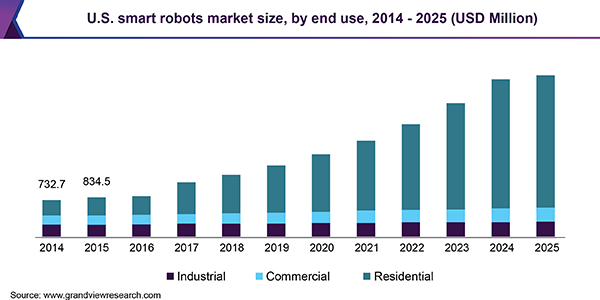
\includegraphics[width=0.4\textwidth]{pics/robotMarket.png}
	\end{center}
	\caption{Robot market size by the end user \cite{b0}}
\end{figure}\\\\
\section{Related Work}
In this section we will briefly discuss other approaches to teach a mobile robot or a computer to play hide and seek.\\
\subsection{Hide and seek - cognitive learning}
Trafton et al. \cite{b1} used hide and seek with a mobile robot and cognitive learning to show, that children are able to learn to play hide and seek 
by learning the features and relations of objects. In order to prove this hypothesis they modeled it in the ACT-R cognitive architecture and 
put the model on a mobile robot to mimic the hiding process of children.
\subsection{Hide and seek - machine learning}
Baker et al. \cite{b2} implemented a multi agent hide and seek game. 
However, this game was implemented on certain constraints and with a map the Agents where trained on, and we wanted our robot 
to work on a more broad and general level. 
Nevertheless, using AI with a mobile robot could serve as an interesting strategy for playing such a hide and seek game.
\subsection{Further algorithms for performing a view search}
We decided to use a depths-first search of the room in order to mimic a child's wandering behavior in a game of hide and seek and leave no corner of the room untouched.
However, LaValle et al. \cite{b3} provided a formal algorithm in order to scan a room for persons, which could be also utilized for a game of hide and seek.\\\\
\section{Methodology}
In the following we will discuss the milestones we set in order to achieve our main goal.
Our main goal was to make Zenbo play the seekers role in a game of hide and seek.
We divided this goal into three main parts:
\begin{itemize}
	\item Navigation (how to move to a certain point in a room)
	\item Computer vision (how to Zenbo detect a person)
	\item Speech recognition (how can we process voice commands from a person)
\end{itemize}
In order to define the project's scope, we created smaller milestones we hoped to hit:
\begin{itemize}
	\item Interact with a human to ask to play hide and seek
	\item Count until a certain number and scan the room
	\item Allow people to give hints by saying the robot's name
	\item Show emotional behavior while searching for people
	\item If the robot sees a face he can recognize if he has met the person before
\end{itemize}
Additionally we added optional goals:
\begin{itemize}
	\item Inverse hide and seek, the people need to search for the robot
	\item Hide and seek in multiple rooms
	\item Intelligent searching of the room instead of a random walk
\end{itemize}
The optional goals served as extended tasks in order to achieve a better usability for a Zenbo hide and seek game and to
supply us with challenges if we had the opportunity to add them at the end of the project.\\
We could not realize two of our milestones, namely:
\begin{itemize}
	\item Allow people to give hints by saying the robot's name
	\item If the robot sees a face he can recognize if he has met the person before
\end{itemize}
This was due drawbacks in the Zenbo SDK and therefore out of our reach.
Also, both milestones turned out to be not game-breaking. See section \ref{sec:drawbacks} for further details.
\\\\
\section{Experimental Setup}
In here we will describe how we programmed Zenbo in order to play a hide and seek game and what the technical specifications 
of Zenbo were. In the end we will discuss difficulties we had and the improvements that could be made on Zenbo.\\
\subsection{Zenbo}
\begin{figure}[h]  \label{fig:zenbopic}
	\begin{center}
		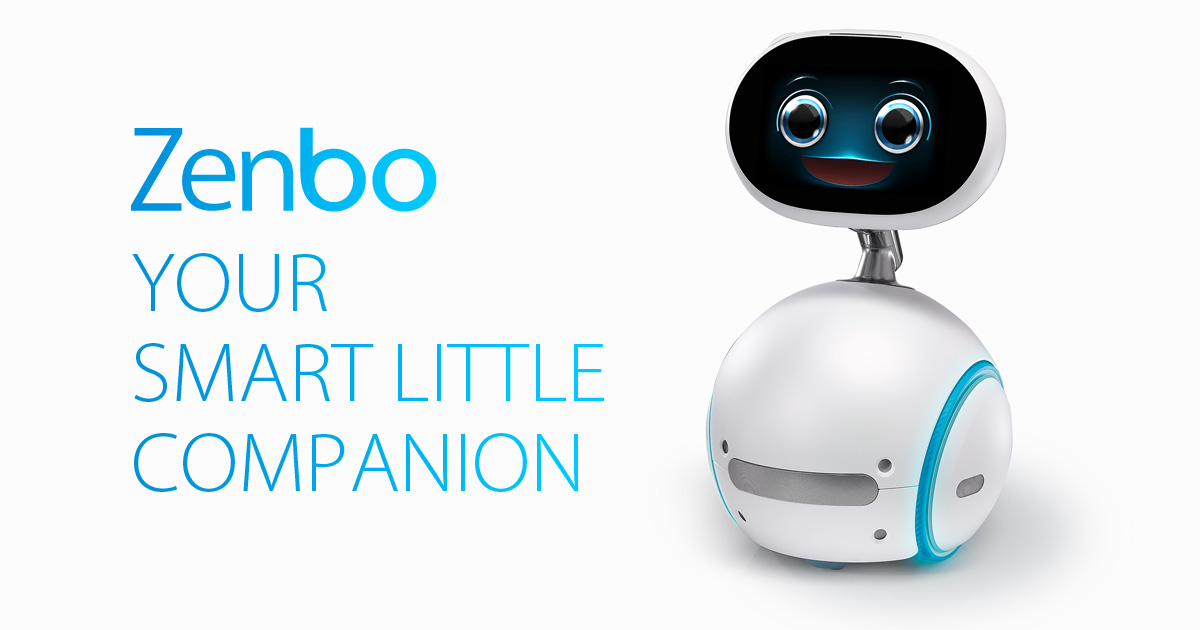
\includegraphics[width=0.5\textwidth]{pics/ZenboPicture.jpg}
	\end{center}
	\caption{Robot market size by the end user}
\end{figure}
Zenbo is a mobile robot designed for interaction with humans, which, according to Asus, can be used for \cite{b6} cite ws:
\begin{itemize}
	\item Innovative Education (As a teaching assistant)
	\item Health \& Safety
	\item Smart Business (As first customer liner)
\end{itemize}
In Table \ref{tab:zenbospecs} the technical specifications of Zenbo are shown. We wanted to utilize Zenbo's camera in order to detect 
people who are hiding. With the drop, range and ultrasonic sensors we wanted to detect whether or not a obstacle is in Zenbo's way in order to avoid it.
\begin{table}[h]\label{tab:zenbospecs}
	\begin{center}
		\begin{tabular}{ll}
			\hline
			Sensor       & Value                                                             \\
			\hline
			OS           & Android (6.0.2 in our case)                                       \\\\
			Memory       & 4GB /                                                             \\\\
			Storage      & 32 GB / 128 GB                                                    \\\\
			Camera       & 3D Camera, 1300 Pixels                                            \\\\
			Connectivity & \begin{tabular}[c]{@{}l@{}}Wi-Fi 802.11AC                         \\ Bluetooth -,BT4.0\\ CIR - 940nm\end{tabular}                                                                                                                          \\\\
			Audio        & High Quality Speaker                                              \\
			Sensor       & \begin{tabular}[c]{@{}l@{}}Touch Sensor – Interactive interface \\ \\ Drop Sensor – Avoid from falling into gaps\\ Range Sensor – Detect forward distance\\ Ultrasonic Sensor – Avoid from obstacles\end{tabular} \\\\
			Battery      & 95W                                                               \\\\
			Standby Time & 18h                                                               \\\\
			Talktime     & 4h                                                                \\\\
			Dimensions   & 37,x 37,x 62,cm (LxWxH)                                           \\\\
			Weight       & 10 kg                                                             \\\\
			\hline \\                                                     
		\end{tabular}
	\end{center}
	\caption{Technical Specifications of Zenbo \cite{b6}}
\end{table}
\subsection{Zenbo functionality}
Zenbos operating system is Android, therefore it requires an Android application in order to run code on it.
The App needs the Zenbo SDK in order to run Zenbo functions. 
The SDK functions can then be accessed over the $RobotAPI$ object. 
In order to instantiate, the object needs the application context and a object called $RobotCallback$.
Actions (like moveTo) can be triggered on the $RobotAPI$ object, while data is asynchronously processed 
through the $RobotCallback$. An illustration of the functionality can be seen in Figure \ref{fig:zenboSDK}. 
\begin{figure}  \label{fig:zenboSDK}
	\begin{center}
		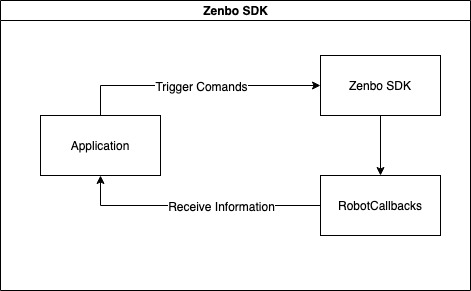
\includegraphics[width=0.45\textwidth]{pics/zenboSDK.jpg}
	\end{center}
	\caption{Illustration of the Zenbo SDK}
\end{figure}
\subsection{Implementation details}
We implemented our code in Java as an Android application and utilized the Zenbo SDK. In the following section
we will discuss how we implemented our three main goals: navigation, computer vision and speech recognition.
Lastly, we will review user interactions with Zenbo.\\
\subsubsection{Navigation}
For navigation, we first needed to figure out how to scan the room properly, so 
a map for movement could be created. Zenbo SDK provides a room scanning functionality, which we utilized.
After scanning the room, the map with all room coordinates could be obtained with the 
function $contacts.room.getAllRoomInfo()$ of the robotAPI.
Next we needed to figure out how to move Zenbo and Zenbo's head. In order to move to a certain position, the Zenbo SDK provides a function called $motion.moveBody$.
This function expects as arguments:
\begin{table}[h]
	\begin{tabular}{lll}
		double & relativeX           & relative movement on the x axis [m] \\
		double & relativeY           & relative movement on the y axis [m] \\
		double & relativeThetaRadian & change of angle of the robot [rad]  \\
		enum   & speedLevel          & how fast the robot should move      
	\end{tabular}
\end{table}\\
In order to move the head of Zenbo to left and right, we utilized a function called $motion.moveHead$.
This function expects the following arguments: 
\begin{table}[h]
	\begin{tabular}{lll}
		float & yawRadian   & how much the head is supposed to be turned [rad] \\
		float & pitchRadian & how much the head is supposed to be turned [rad] \\
		enum  & speedLevel  & how fast the robot should move  its head         
	\end{tabular}
\end{table}\\
From those two methods we created our wrappers: $moveHeadLeft$, $moveHeadRight$, $moveHeadCenter$ 
and $goToLocation$.
$goToLocation$ takes as an argument one $Intpoint$, which was our representation of a Point in the coordinate system.
The other methods we created need no further attributes.\\
The next task we needed to fulfill was to search for people. Therefore we performed a depth first search (DFS).
DFS is more suitable for this kind of problem, because the breath of the search tree was in our case $4^n$, 
so the tree would get very big in only a few steps. In addition, we wanted to further mimic a child searching for another and
children tend to exhaust searching one location before moving on to another, 
instead of slowly moving away from their position keeping track of every possible position around them.
Figure \ref{fig:dfs_vsbfs} illustrates this issue quite well.
% DFS_VS_BFS
\begin{figure}[h]  \label{fig:dfs_vsbfs}
	\begin{center}
		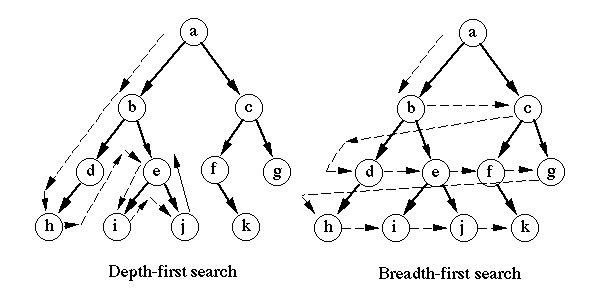
\includegraphics[width=0.4\textwidth]{pics/DFS_VS_BFS.png}
	\end{center}
	\caption{State diagramm of the search process}
\end{figure}\\
The deterministic final automata that describes our search can be seen in figure \ref{fig:zenboSeek}. \\
So after counting until a fixed number, Zenbo starts to perform a DFS around the room.
At every new position he moves his head to the left and to the right, in order to grasp more information about his environment, before moving on. In case he detected a person by 
his computer vision module, he calls out the hider's name and checks their face. If he finds the hider Zenbo stops.
% ZenboSeek
\begin{figure}[h]  \label{fig:zenboSeek}
	\begin{center}
		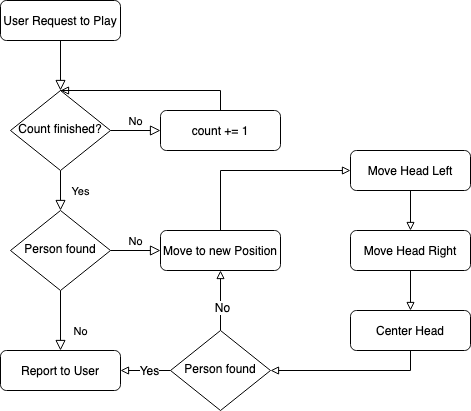
\includegraphics[width=0.4\textwidth]{pics/ZenboSeek.png}
	\end{center}
	\caption{State diagram of the search process}
\end{figure}
If the room does not have an endless number of points and the user is in the room, 
the problem will be solvable this way, because the robot will just visit every point of the room and look around, and 
if he does not detect any person the robot will move on.
LaValle et al. \cite{b3} described a more efficient way, which requires cutting the room into sections in order to find a target.
But we decided that the brute force solution was simpler and would make for a more fun for game, as the game would last longer.\\
Different solution techniques could be applied in future implementations in order to get a level system.
\subsubsection{Computer Vision}
We needed to combine computer vision with a learning algorithm in order to detect whether or not the robot has a person in front of it.
We first tried to access the camera, but found out that Zenbo SDK only provides an already preprocessed face detection. So we decided to utilize this.\\
In order to detect a persons face, the method $vision.requestDetectFace$ on the robotAPI needs to be called. This method requests a object, called $FaceDetectConfig$.
in FaceDetectConfig, the following parameters can be adjusted: 
\begin{table}[h]
	\begin{tabular}{lll}
		int  & interval           & how often to check for faces                 \\
		bool & enableDebugPreview & \begin{tabular}[c]{@{}l@{}}show a preview of \\the detected face for debug purposes\end{tabular} \\
		bool & enableDetectHead   & detect the persons face                      \\
		bool & enableFacePosture  & detect where the user is looking             \\
		bool & enableCandidateObj & allows detection of person like things       \\
		int  & intervalInMS       & timespan of one interval [ms]                \\
	\end{tabular}
\end{table}\\
In the robot callback the results can be obtained from a function called $onDetectFaceResult$.
This method returns a list of objects, named $DetectFaceResult$, which contains all information about the detected faces.
The only attribute from $DetectFaceResult$ that is in our interest is @TODO DAVID, since we only want to compare the appearance of two people.\\
Figure \ref{fig:computerVision} shows the states that are possible when detecting a person. If $onDetectFaceResult$ is called, whether or not 
the robot is in seeking mode is checked. In case the robot is in seeking mode, the UUID gets compared and if the person is in front of the robot, Zenbo makes a happy face
and says: \textit{'I found you! \{name\}'}. If Zenbo is searching for people to play hide and seek with him, he refuses to play with a group, but 
in case of one person, he asks the person if she wants to play with him. In case the person confirms Zenbo counts until a fixed number and then searches for the user.
\begin{figure}[h]  \label{fig:computerVision}
	\begin{center}
		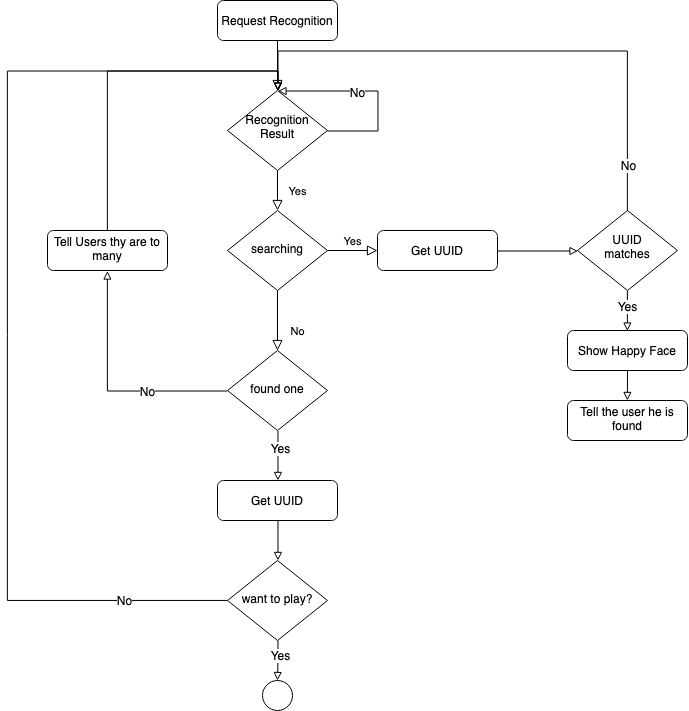
\includegraphics[width=0.4\textwidth]{pics/computerVisionFlow.png}
	\end{center}
	\caption{State diagram for detecting people}
\end{figure}
\subsubsection{Speech recognition} \label{sec:speechreconition}
Speech recognition is a interdisciplinary subfield of computer linguistics, that enables and develops methodologies and techniques in order to process 
natural language towards written text. \cite{b4}  Applications can be found in smart home assistants or on smartphones.
For our speech recognition task we used the Zenbo SDK. The SDK provides a callback called $onEventUserUtterance$, in which a JSONObject can be found.
From this JSONObject, we got the sub-object 'event\_user\_utterance' and from there we took the string: 'user\_utterance'. This string 
corresponds to the sentence formulated by the user and parsed internally by the zenboSDK.\\
Accordingly towards the state shown Figure \ref{fig:zenboSpeech} we parse the users answer.
In order to be more user friendly we assured that Zenbo can understand multiple positive and negative answers:
\begin{itemize}
	\item Yes: "Yes", "sure", "I do", ...
	\item No: "no", "I do not", "I don't", ...
\end{itemize}
The lists for yes and no could be extended by far more expressions but we limited ourselves to those three.\\
\begin{figure}  \label{fig:zenboSpeech}
	\begin{center}
		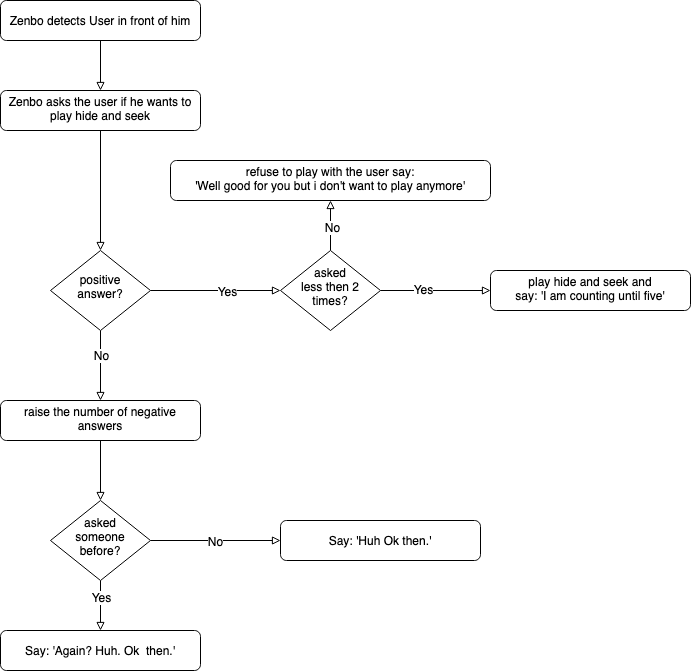
\includegraphics[width=0.4\textwidth]{pics/ZenboSpeech.png}
	\end{center}
	\caption{State diagram for speech recognition and user interaction}
\end{figure}\\
\subsubsection{User Interaction}
In order to interact with the user, we utilized the speech recognition described in Section \ref{sec:speechreconition}. We wanted to 
interact with natural language instead of a touch screen in order to create a more natural user experience.
So on a user command, we could reply via a function in the Zenbo SDK called: $robot.speakAndListen$. This first made the robot speak the sentence we 
gave him, and afterwards triggered the voice in order to wait for user input.\\
The two other ways how we handled communication with the user were setting the light of the weels to different colors in order to express the robots feelings and 
by moving the robots head. With those methods we wanted to express the robot's emotions in order to have the user feel better connected to him.\\
We also wanted to create some sort of emotions by having Zenbo be offended after two refusals to play hide and seek with him, as visible in Figure \ref{fig:zenboSpeech}
\\\\
\section{Results}
In this section we will cover the results of our implementation and the difficulties we had.
First, we will talk about the features we could not implement because Asus did not gave us the ability. 
Next, we will talk about the drawbacks we experienced while using the Zenbo SDK, and at the end, we will make some suggestions for improvements which could be made on the Zenbo SDK.
\subsection{Features we could not realize} \label{sec:drawbacks}
\subsubsection{People giving hints by speaking}
We wanted Zenbo to listen to its environment while moving around and searching for the user. In case the user makes a sound or shouts 'Zenbo I am here', 
Zenbo would rather search in that direction. An interesting scenario would then be caused by the situation if two people shout at the same time 'Zenbo I am here'.
Then either Zenbo could memorize both locations and search for them or pretend like he is confused and start searching somewhere else.\\
We also thought that it would be possible to achieve this goal since Asus claims that: 
"[...] Zenbo is equipped with microphones, therefore apart from being able to receive sounds, it is also capable of determining the direction where sounds are coming from.". \cite{b5}
But we were not able to find such a functionality in the Zenbo SDK.
\subsubsection{The robot can remember a face he has seen before}
In order to achieve this we wanted to store the UUID of the face of the person Zenbo has played with and if the person showed up again, we wanted to
react to this person accordingly (for instance, ask for the persons name and if the person shows up again greet them with that name).
But here the face recognition turned out to be very imprecise, and as we were unable to get access to the camera to perform our own categorization with images of players, we also could not realize this feature.
\subsection{Issues while the project}
In this section we wanted to summarize the issues we had while realizing the project. We again grouped them in our 
main three goals: Navigation, computer vision and language processing.
\subsubsection{Navigation}
For the navigation part Zenbo needs to create a map of the room, in order to give the maps coordinates back from the $contacts.room.getAllRoomInfo()$ method.\\
We found out that we need admin rights in the Zenbo controller which we did not have. Therefore, we tried different emails together with the TAs 
and came to the conclusion that the best would be to factory reset Zenbo. Because we have reset Zenbo we ran into Google's factory reset protection.
Google's factory reset protection locks a smartphone (or any other android device after Android 5) 
after it is factory reset and requires it to insert the email of the previous owner. 
Nevertheless we did not have the email, so this problem was close to crash the whole project.\\
We want to thank the TAs at this point for helping us with Zenbo and that they finally managed to rerun the Robot.
\subsubsection{Computer Vision}
Here we had the problem that Zenbo sometimes just could not detect a face and return the id $-15$. 
It looks like this was an internal bug, so we had to surmount this problem by filtering out all samples with $-15$.
This of course then decreased the rate of people we were able to detect.
The Zenbo SDK does not provide a method to get the current camera output (even though this would really be feasible on any other app-running device),
therefore we could not implement our own model for facial detection. That is really sad because with the development of Firebase, Google provides
really good ML models in order to detect a face and tell the difference between two persons.
\subsubsection{Language processing}
For language processing we encountered a problem very similar to that of computer vision. Sometimes the processed language was definitely not 
what we were saying to the robot. Also, the Zenbo's language processing in general felt very slow and not very intuitive, as it does with Siri or Google.
This sadly decreased the positive experience a user would have with Zenbo and our App and it's a shame something so simple stands in the way of a positive user interaction.
Again, here it would have been great to provide a callback with a stream of the robot's microphone so that the NLP could be done by a external library.

\subsection{Improvements of the Zenbo SDK}
As mentioned above the main improvements on the Zenbo SDK we would suggest are to let the user manually choose a method for face and speech recognition, so that Apps could evolve together with the state-of-the-art instead of them having to wait for Asus internally updating the technology.\\
An other thing that we really suffered from while developing with the Zenbo SDK was the bad documentation of the accessible methods.
It would be great for developers to see a website with technical examples of how certain functions could be applied instead of just having one large project with 10 examples available.\\\\
\section{Conclusion}
Mobile robots will definitely play an increasing role in the future in end user households. 
They can be extremely useful and entertaining for people of every age. Asus Zenbo and Asus Zenbo Junior
have the advantage that end users as well as companies are able to create applications for them.
Therefore, they serve a stepping stone in the increasing use of mobile robots by end users.
With our hide and seek game we tried to give ourselves a challenging task based on the requirements of a possible end user of Zenbo.
Besides the few drawbacks we had while developing the App, it still was an interesting project and we learned a lot in the field of robotics
with Zenbo.\\\\ 
\section*{Acknowledgment}
We would like to thank Professor Fu and the teaching assistants for the opportunity they gave us with this project.
Thank you for helping us with all the questions we had while our project and especially thank you for repairing Zenbo after the factory reset.\\
\begin{thebibliography}{00}
	\bibitem{b0} https://www.grandviewresearch.com/industry-analysis/smart-robots-market
	\bibitem{b1} J. Gregory Trafton, J. Gregory Trafton, Dennis Perznowski: Children and robots learning to play hide and seek
	\bibitem{b2} Bowen Baker, Ingmar Kanitscheider, Todor Markov: Emergent Tool Use From Multi-Agent Autocurricula
	\bibitem{b3} Steven M. LaValle: PLANNING ALGORITHMS
	\bibitem{b4}  ""
	\bibitem{b5} https://zenbo.asus.com/developer/documents/Design-Guideline/Zenbo-Introduction/Basic-Functions
	\bibitem{b6} https://www.asus.com/Commercial-Intelligent-Robot/Zenbo/
\end{thebibliography}
\vspace{12pt}
\end{document}
